\documentclass[a4paper,11pt]{beamer}
\usepackage{etex}
\usepackage{lmodern}
\usepackage[french]{babel}
\usepackage[T1]{fontenc}
\usepackage[utf8]{inputenc}
% \usepackage{listings}
\usepackage{graphicx} 
\usepackage{ragged2e}  
% \usepackage{array}
% \usepackage{tikz} 
% \usepackage{pgf-umlcd} 
%\usepackage{csquotes}
\usepackage[pdf]{pstricks}
\usepackage{pst-sigsys}
\usepackage{amsmath,amsfonts,bm}
\usepackage{pstricks-add}
% \usepackage{physics}
% \usepackage{ulem}
% \usepackage{wasysym}
% \usepackage{hyperref}
% \usepackage{color}
\usepackage{fontawesome}
\setbeamertemplate{navigation symbols}{}  
 
\usetheme{Darmstadt}
\setbeamertemplate{footline}{\insertframenumber/\inserttotalframenumber}
\title{M1 IEAP - BTI/FH/IEMH\\pFIEA02CM : Analyse et Traitement du Signal}
\author{Flavy ROSEREN\\Martin EGIZIANO\\Frank BULOUP}
\institute{Aix Marseille Université\\Institut des Sciences du Mouvement}
\date{}

\setbeamertemplate{footline} 
{  
	\begin{beamercolorbox}[ht=2.5ex,dp=1.125ex,%
      leftskip=.3cm,rightskip=.3cm plus1fil]{title in head/foot}%
      {\usebeamerfont{title in head/foot}\insertshorttitle} \hfill    
      \insertframenumber / \inserttotalframenumber%
    \end{beamercolorbox}%
%     \begin{beamercolorbox}[colsep=1.5pt]{lower separation line foot}
%     \end{beamercolorbox} 
}

% \newcounter{exerciceBlocNumber}
%    \newcommand{\exerciceNumber}{\stepcounter{exerciceBlocNumber} 
%   				Exercice \arabic{exerciceBlocNumber}.} 

\newcounter{exampleBlockCounter}
\setcounter{exampleBlockCounter}{1}


\begin{document} 
 
\begin{frame}[plain] 
	\titlepage \center{
\includegraphics[scale=0.75]{images/by-nc-sa.eps}}
	\vspace{1cm}
	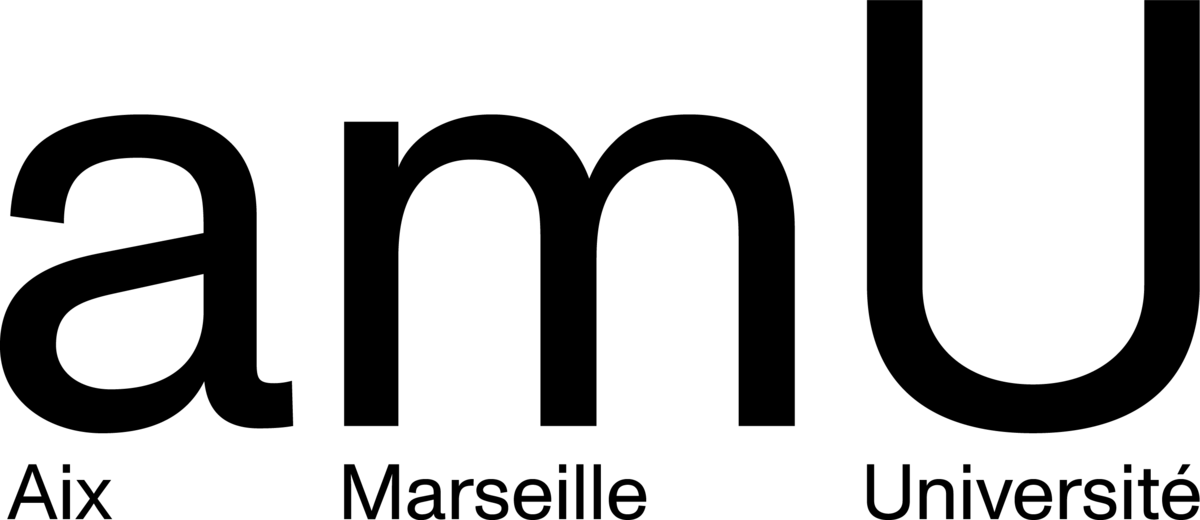
\includegraphics[scale=0.6]{images/LogoAMU.png}\hspace*{2cm}
	
\includegraphics[scale=0.2]{images/LogoCNRS.eps}\hspace*{2cm}
	
\includegraphics[scale=0.1]{images/LogoISM.eps}
\end{frame} 

\begin{frame}[plain]{Organisation du cours}
\begin{itemize}
	\item Deux parties : signal et système
	\item Séances en salle informatique (E207, D217, TPR1 00.11)
	\item Présentation des notions théoriques
	\item Applications pratiques sur papier ou sur Python
	\item Contrôle continu à mi-parcours d'une demie heure ($40\%$)
	\begin{itemize}
	    \item \faWarning\, Attention: contrôles continus possibles en début de séance
	\end{itemize}
	\item Un examen final d'une heure ($60\%$)
\end{itemize}
\end{frame}

\begin{frame}[plain]{Références}
\begin{itemize}
\item AMETICE !
\item Matlab : licence etudiants AMU
\item Octave GNU (alternative à Matlab)
		\url{http://octave.sourceforge.net}
\item\normalsize{La webtv de l'enseignement supérieur}
		\url{http://www.canal-u.tv}
\begin{itemize}
	\item Chapitre "Leçons de choses" - Partie 4 (Trigo) :
	\href{https://www.canal-u.tv/chaines/canal-unisciel/lecons-de-choses/chapitre-lecons-de-choses-partie-4-formules-de}{lien}
	\item Nombres complexes - Parties $1$ à $4$ + exercices : 
	\href{https://www.canal-u.tv/chaines/canal-unisciel/nombres-complexes}{lien}
\end{itemize}		
\item\normalsize{Quelques liens utiles :}
\begin{itemize}
	\item \href{http://www.dspguru.com}{DSP Guru}
	\item \href{http://www.dspguide.com/pdfbook.html}{DSP Guide}
	\item \href{https://ocw.mit.edu/courses/electrical-engineering-and-computer-science/6-003-signals-and-systems-fall-2011/index.htm}{MIT 6-003}
\end{itemize}	
\end{itemize}
\end{frame}

\begin{frame}[plain]
\frametitle{Objectifs de cette formation}
\center
À l'issue de cette formation, vous serez capable de :
    \vspace{0.25cm}

\begin{enumerate}
    \item Expliquer la différence entre Signal Continu et Signal Discret
    \item Utiliser la représentation temporelle d'un signal discret
 		\begin{itemize}
 		  \item Décrire les concepts d'échantillon et de période d'échantillonnage
 		  \item Créer le vecteur temporel associé aux données
 		  \item Représenter graphiquement les données
 		\end{itemize}
  \item Utiliser la représentation fréquentielle d'un signal
  	    \begin{itemize}
  	      \item Décrire les concepts de Spectres monolatéral ou bilatéral
  	      \item Expliquer le rôle de la "Transformée de Fourier Rapide"
  	      \item Créer le vecteur fréquentiel associé à la TFR d'un signal
 		  \item Représenter et interpréter graphiquement cette TFR
 		\end{itemize}
 \item Appliquer un filtre numérique prédéterminé sur un signal
\end{enumerate}
\end{frame}

\begin{frame}
	\begin{center}
		\textbf{\textcolor{red}{Pourquoi étudier le traitement du signal ?}}
	\end{center}
	\pause
	\begin{block}{
\includegraphics[scale=0.45]{images/Logo_Wikipedia.eps}
	\enspace Définition} Le traitement du signal est la discipline qui développe et
	étudie les techniques de traitement, d'analyse et d'interprétation des signaux
	\end{block}
	\pause
	\begin{center}
		\textbf{\textcolor{red}{C'est donc forcément utile en analyse du mouvement :
		\\
		\smallbreak 
		après acquisition, enregistrement des signaux,\\ il faut bien
		passer à l'analyse !\\
		\bigbreak
		 Acquisition des signaux - Métrologie : FPS620BM}}
	\end{center}
\end{frame}

\begin{frame}{Première Partie}
	\tableofcontents
\end{frame}

\section{Rappels de Mathématique} 
\subsection{Trigonométrie}
\begin{frame}
	\begin{block}{Pourquoi des rappels de trigonométrie ?}
	La trigonométrie est utilisée dans de nombreuses sciences :
	\itemize
	  \item physique
	  \item mécanique
	  \item électricité
	  \item \ldots et en \ldots
	  \item \textbf{\textcolor{red}{traitement du signal}}
	\end{block}
	\pause
	\begin{block}{
\includegraphics[scale=0.45]{images/Logo_Wikipedia.eps}
	\enspace Qu'est-ce que la trigonométrie ?}
	\begin{center}
		Du grec \textit{trigonos} (triangulaire) et \textit{métron} (mesure)\\
		\smallbreak
		Branche des mathématiques qui traite des \textbf{\textcolor{red}{relations}}
		entre\\
		\textbf{\textcolor{red}{distances et angles}} dans les
		\textbf{\textcolor{red}{triangles}} et des \textbf{\textcolor{red}{fonctions
		\\trigonométriques}} telles que sinus, cosinus et tangente
	\end{center}
	
	\end{block}
\end{frame}
\begin{frame}
	\begin{block}{Théorème de Pythagore}
		Dans un triangle rectangle, le carré de la longueur de l'hypoténuse est égal
		à la somme des longueurs des carrés des deux autres côtés
	\end{block}
	\begin{figure}
		\begin{pspicture}[showgrid=false](0,0)(6,4)
			\psline(0,0)(0,4)(6,0)(0,0)
			\psline(0,0.5)(0.5,0.5)(0.5,0)
			\rput(4.35,2.25){$c$ : hypoténuse}
			\rput(5.95,1.75){(côté opposé à l'angle droit)}
			\rput(-.25,2){$a$}
			\rput(3,-.25){$b$}
		\end{pspicture}
	\end{figure}
	\[
	\begin{aligned}
	c^2 = a^2 + b^2 \Leftrightarrow
		c = \sqrt{a^2 + b^2}
	\end{aligned}\]
\end{frame}
\begin{frame}
	\begin{block}{Quelques formules de trigonométrie}
	\[
	\begin{aligned}
		cos(\theta) &= \frac{a}{c}\\
		sin(\theta) &= \frac{b}{c}\\
		tan(\theta) &= \frac{sin(\theta)}{cos(\theta)} = \frac{b}{a}
	\end{aligned}\]
	\end{block}
	\begin{figure}
		\psset{unit=0.75cm}
		\begin{pspicture}[showgrid=false](0,0)(6,4)
			\psline(0,0)(0,4)(6,0)(0,0)
			\psline(0,0.5)(0.5,0.5)(0.5,0)
			\rput(3.35,2.25){$c$}
			\rput(-.25,2){$a$}
			\rput(3,-.25){$b$}
			\rput(0.5,2.85){$\theta$}
			\psarc(0,4){1}{-90}{-34}
		\end{pspicture}
	\end{figure}
\end{frame}

\begin{frame}
	\begin{exampleblock}{Exercice \Roman{exampleBlockCounter} - Trigonométrie}
		\begin{enumerate}
			  \item Placer les angles remarquables suivants sur le cercle trigonométrique
			  : $0$, $\pi$, $\frac{\pi}{2}$, $\frac{\pi}{4}$, $\frac{\pi}{3}$, 
			  $\frac{2\pi}{3}$ et $\frac{\pi}{6}$
			  \item Donner les valeurs des cosinus et sinus des angles précédents
			  \item Montrer que $cos^2(\theta) + sin^2(\theta) = 1$
			  \item Exprimer $cos(-\theta)$, $sin(-\theta)$, $cos(\theta +
			  \frac{\pi}{2})$, $sin(\theta - \frac{\pi}{2})$, $cos(\theta - \pi)$,
			  $sin(\theta + \pi)$ en fonction de $cos(\theta)$ ou $sin(\theta)$
		\end{enumerate}
	\end{exampleblock}\stepcounter{exampleBlockCounter}
\end{frame}
%0
\begin{frame}
\begin{block}{La fonction Cosinus}
\begin{figure}
	\psset{unit=1cm}
	\begin{pspicture}[showgrid=false](0,0)(10,4)
		\pscircle[linewidth=1pt](1.5,1.5){1.5}
		\psline{->}(4,1.5)(10,1.5)	
		\psline{->}(4,0)(4,3.25)		
		\rput(4,3.5){$cos(\theta)$}
		\rput(10.2,1.25){{$\theta$}}
		
		\psline[linecolor=red]{<->}(1.5,1.5)(3,1.5)	
		\rput(1.5,1){$\theta=0$}					
		\rput(1.5,3.5){$cos(\theta)=1$}	
		\pause			
		\psdot*[linecolor=red](4,3)
		\rput(4.15,1.25){\textcolor{red}{$0$}}
		\rput(3.75,3){\textcolor{red}{$1$}}
	\end{pspicture}
\end{figure}
\end{block}
\end{frame}
%pi/6
\begin{frame}
\begin{block}{La fonction Cosinus} 
\begin{figure}
	\psset{unit=1cm}
	\begin{pspicture}[showgrid=false](0,0)(10,4)
		\pscircle[linewidth=1pt](1.5,1.5){1.5}
		\psline{->}(4,1.5)(10,1.5)	
		\psline{->}(4,0)(4,3.25)			
		\rput(4,3.5){$cos(\theta)$}
		\rput(10.2,1.25){{$\theta$}}
		\psdot*[linecolor=black](4,3)

		\psline[linecolor=black](2.79903810567666,1.5)(3,1.5)
		\psline[linecolor=black](1.5,1.5)(2.79903810567666,2.25)
		\psline[linecolor=red]{<->}(1.5,1.5)(2.79903810567666,1.5)
		\psline[linecolor=brown,linestyle=dashed](2.79903810567666,2.25)(2.79903810567666,1.5)
		\psarc[linecolor=black,arcsepB=2pt,linewidth=2pt]{->}(1.5,1.5){1.5}{0}{30}
		\rput(3.25,2){\textcolor{black}{$\theta$}}

		\rput(1.5,1){$\theta=\frac{\pi}{6}$}					
		\rput(1.5,3.5){$cos(\theta)=\frac{\sqrt{3}}{2}$}	
		\pause			
		\psdot*[linecolor=red](4.5235987755983,2.779)
		\rput(4.5235987755983,1.15){\textcolor{red}{$\frac{\pi}{6}$}}
		\psline[linecolor=red](4.5235987755983,1.6)(4.5235987755983,1.4)
		\rput(3.65,2.779){\textcolor{red}{$\frac{\sqrt{3}}{2}$}}
		\psline[linecolor=red](3.9,2.779)(4.1,2.779)
		
	\end{pspicture}
\end{figure} 
\end{block}
\end{frame}
%pi/4
\begin{frame}
\begin{block}{La fonction Cosinus}
\begin{figure}
	\psset{unit=1cm}
	\begin{pspicture}[showgrid=false](0,0)(10,4)
		\pscircle[linewidth=1pt](1.5,1.5){1.5}
		\psline{->}(4,1.5)(10,1.5)	
		\psline{->}(4,0)(4,3.25)			
		\rput(4,3.5){$cos(\theta)$}
		\rput(10.2,1.25){{$\theta$}}
		\psdot*[linecolor=black](4,3)
		\psdot*[linecolor=black](4.5235987755983,2.779)

		\psline[linecolor=black](2.55,1.5)(3,1.5)
		\psline[linecolor=black](1.5,1.5)(2.55,2.55)
		\psline[linecolor=red]{<->}(1.5,1.5)(2.55,1.5)
		\psline[linecolor=brown,linestyle=dashed](2.55,2.55)(2.55,1.5)
		\psarc[linecolor=black,arcsepB=2pt,linewidth=2pt]{->}(1.5,1.5){1.5}{0}{45}
		\rput(3.25,2){\textcolor{black}{$\theta$}}
		
		\rput(1.5,1){$\theta=\frac{\pi}{4}$}					
		\rput(1.5,3.5){$cos(\theta)=\frac{\sqrt{2}}{2}$}	
		\pause			
		\psdot*[linecolor=red](4.78539816339745,2.5607)
		\rput(4.78539816339745,1.15){\textcolor{red}{$\frac{\pi}{4}$}}
		\psline[linecolor=red](4.78539816339745,1.6)(4.78539816339745,1.4)
		\rput(3.65,2.5607){\textcolor{red}{$\frac{\sqrt{2}}{2}$}}
		\psline[linecolor=red](3.9,2.5607)(4.1,2.5607)
		
	\end{pspicture}
\end{figure} 
\end{block}
\end{frame}
%pi/3
\begin{frame}
\begin{block}{La fonction Cosinus}
\begin{figure}
	\psset{unit=1cm}
	\begin{pspicture}[showgrid=false](0,0)(10,4)
		\pscircle[linewidth=1pt](1.5,1.5){1.5}
		\psline{->}(4,1.5)(10,1.5)	
		\psline{->}(4,0)(4,3.25)			
		\rput(4,3.5){$cos(\theta)$}
		\rput(10.2,1.25){{$\theta$}}
		\psdot*[linecolor=black](4,3)
		\psdot*[linecolor=black](4.5235987755983,2.779)
		\psdot*[linecolor=black](4.78539816339745,2.5607)

		\psline[linecolor=black](2.25,1.5)(3,1.5)
		\psline[linecolor=black](1.5,1.5)(2.25,2.79903810567666)
		\psline[linecolor=red]{<->}(1.5,1.5)(2.25,1.5)
		\psline[linecolor=brown,linestyle=dashed](2.25,2.79903810567666)(2.25,1.5)
		\psarc[linecolor=black,arcsepB=2pt,linewidth=2pt]{->}(1.5,1.5){1.5}{0}{60}
		\rput(3.25,2){\textcolor{black}{$\theta$}}
		
		\rput(1.5,1){$\theta=\frac{\pi}{3}$}					
		\rput(1.5,3.5){$cos(\theta)=\frac{1}{2}$}	
		\pause			
		\psdot*[linecolor=red](5.0471975511966,2.25)
		\rput(5.0471975511966,1.15){\textcolor{red}{$\frac{\pi}{3}$}}
		\psline[linecolor=red](5.0471975511966,1.6)(5.0471975511966,1.4)
		\rput(3.65,2.25){\textcolor{red}{$\frac{1}{2}$}}
		\psline[linecolor=red](3.9,2.25)(4.1,2.25)
		
	\end{pspicture}
\end{figure} 
\end{block}
\end{frame}
%pi/2
\begin{frame}
\begin{block}{La fonction Cosinus}
\begin{figure}
	\psset{unit=1cm}
	\begin{pspicture}[showgrid=false](0,0)(10,4)
		\pscircle[linewidth=1pt](1.5,1.5){1.5}
		\psline{->}(4,1.5)(10,1.5)	
		\psline{->}(4,0)(4,3.25)			
		\rput(4,3.5){$cos(\theta)$}
		\rput(10.2,1.25){{$\theta$}}
		\psdot*[linecolor=black](4,3)
		\psdot*[linecolor=black](4.5235987755983,2.779)
		\psdot*[linecolor=black](4.78539816339745,2.5607)
		\psdot*[linecolor=black](5.0471975511966,2.25)

		\psline[linecolor=black](1.5,1.5)(3,1.5)
		\psline[linecolor=black](1.5,1.5)(1.5,3)
		\psarc[linecolor=black,arcsepB=2pt,linewidth=2pt]{->}(1.5,1.5){1.5}{0}{90}
		\rput(3.25,2){\textcolor{black}{$\theta$}}
		
		\rput(1.5,1){$\theta=\frac{\pi}{2}$}					
		\rput(1.5,3.5){$cos(\theta)=0$}	
		\pause			
		\psdot*[linecolor=red](5.5707963267949,1.5)
		\rput(5.5707963267949,1.15){\textcolor{red}{$\frac{\pi}{2}$}}
		\psline[linecolor=red](5.5707963267949,1.6)(5.5707963267949,1.4)
		\rput(3.65,1.5){\textcolor{red}{$0$}}
		\psline[linecolor=red](3.9,1.5)(4.1,1.5)
		
	\end{pspicture}
\end{figure} 
\end{block}
\end{frame}
%2pi/3
\begin{frame}
\begin{block}{La fonction Cosinus}
\begin{figure}
	\psset{unit=1cm}
	\begin{pspicture}[showgrid=false](0,0)(10,4)
		\pscircle[linewidth=1pt](1.5,1.5){1.5}
		\psline{->}(4,1.5)(10,1.5)	
		\psline{->}(4,0)(4,3.25)			
		\rput(4,3.5){$cos(\theta)$}
		\rput(10.2,1.25){{$\theta$}}
		\psdot*[linecolor=black](4,3)
		\psdot*[linecolor=black](4.5235987755983,2.779)
		\psdot*[linecolor=black](4.78539816339745,2.5607)
		\psdot*[linecolor=black](5.0471975511966,2.25)
		\psdot*[linecolor=black](5.5707963267949,1.5)

		\psline[linecolor=black](1.5,1.5)(3,1.5)
		\psline[linecolor=black](1.5,1.5)(0.75,2.79903810567666)
		\psline[linecolor=brown,linestyle=dashed](0.75,2.79903810567666)(0.75,1.5)
		\psline[linecolor=red]{<->}(0.75,1.5)(1.5,1.5)
		\psarc[linecolor=black,arcsepB=2pt,linewidth=2pt]{->}(1.5,1.5){1.5}{0}{120}
		\rput(3.25,2){\textcolor{black}{$\theta$}}
		
		\rput(1.5,1){$\theta=\frac{2\pi}{3}$}					
		\rput(1.5,3.5){$cos(\theta)=\frac{-1}{2}$}	
		\psdot*[linecolor=red](6.0943951023932,0.75)
		\rput(6.0943951023932,1.9){\textcolor{red}{$\frac{2\pi}{3}$}}
		\psline[linecolor=red](6.0943951023932,1.6)(6.0943951023932,1.4)
		\rput(3.65,0.75){\textcolor{red}{$\frac{-1}{2}$}}
		\psline[linecolor=red](3.9,0.75)(4.1,0.75)
		
	\end{pspicture}
\end{figure} 
\end{block}
\end{frame}
%3pi/4
\begin{frame}
\begin{block}{La fonction Cosinus}
\begin{figure}
	\psset{unit=1cm}
	\begin{pspicture}[showgrid=false](0,0)(10,4)
		\pscircle[linewidth=1pt](1.5,1.5){1.5}
		\psline{->}(4,1.5)(10,1.5)	
		\psline{->}(4,0)(4,3.25)			
		\rput(4,3.5){$cos(\theta)$}
		\rput(10.2,1.25){{$\theta$}}
		\psdot*[linecolor=black](4,3)
		\psdot*[linecolor=black](4.5235987755983,2.779)
		\psdot*[linecolor=black](4.78539816339745,2.5607)
		\psdot*[linecolor=black](5.0471975511966,2.25)
		\psdot*[linecolor=black](5.5707963267949,1.5)
		\psdot*[linecolor=black](6.0943951023932,0.75)

		\psline[linecolor=black](1.5,1.5)(3,1.5)
		\psline[linecolor=black](1.5,1.5)(0.43933982822017,2.56066017177983)
		\psline[linecolor=brown,linestyle=dashed](0.43933982822017,2.56066017177983)(0.43933982822017,1.5)
		\psline[linecolor=red]{<->}(0.43933982822017,1.5)(1.5,1.5)
		\psarc[linecolor=black,arcsepB=2pt,linewidth=2pt]{->}(1.5,1.5){1.5}{0}{135}
		\rput(3.25,2){\textcolor{black}{$\theta$}}
		
		\rput(1.5,1){$\theta=\frac{3\pi}{4}$}					
		\rput(1.5,3.5){$cos(\theta)=\frac{-\sqrt{2}}{2}$}	
		\psdot*[linecolor=red](6.35619449019235,0.4395)
		\rput(6.35619449019235,1.9){\textcolor{red}{$\frac{3\pi}{4}$}}
		\psline[linecolor=red](6.35619449019235,1.6)(6.35619449019235,1.4)
		\rput(3.55,0.4395){\textcolor{red}{$\frac{-\sqrt{2}}{2}$}}
		\psline[linecolor=red](3.9,0.4395)(4.1,0.4395)
		
	\end{pspicture}
\end{figure} 
\end{block}
\end{frame}
%5pi/6
\begin{frame}
\begin{block}{La fonction Cosinus}
\begin{figure}
	\psset{unit=1cm}
	\begin{pspicture}[showgrid=false](0,0)(10,4)
		\pscircle[linewidth=1pt](1.5,1.5){1.5}
		\psline{->}(4,1.5)(10,1.5)	
		\psline{->}(4,0)(4,3.25)			
		\rput(4,3.5){$cos(\theta)$}
		\rput(10.2,1.25){{$\theta$}}
		\psdot*[linecolor=black](4,3)
		\psdot*[linecolor=black](4.5235987755983,2.779)
		\psdot*[linecolor=black](4.78539816339745,2.5607)
		\psdot*[linecolor=black](5.0471975511966,2.25)
		\psdot*[linecolor=black](5.5707963267949,1.5)
		\psdot*[linecolor=black](6.0943951023932,0.75)
		\psdot*[linecolor=black](6.35619449019235,0.4395)

		\psline[linecolor=black](1.5,1.5)(3,1.5)
		\psline[linecolor=black](1.5,1.5)(0.20096189432334,2.25)
		\psline[linecolor=brown,linestyle=dashed](0.20096189432334,2.25)(0.20096189432334,1.5)
		\psline[linecolor=red]{<->}(0.20096189432334,1.5)(1.5,1.5)
		\psarc[linecolor=black,arcsepB=2pt,linewidth=2pt]{->}(1.5,1.5){1.5}{0}{150}
		\rput(3.25,2){\textcolor{black}{$\theta$}}
		
		\rput(1.5,1){$\theta=\frac{5\pi}{6}$}					
		\rput(1.5,3.5){$cos(\theta)=\frac{-\sqrt{3}}{2}$}	
		\psdot*[linecolor=red](6.6179938779915,0.23)
		\rput(6.6179938779915,1.9){\textcolor{red}{$\frac{5\pi}{6}$}}
		\psline[linecolor=red](6.6179938779915,1.6)(6.6179938779915,1.4)
		\rput(3.55,0.23){\textcolor{red}{$\frac{-\sqrt{3}}{2}$}}
		\psline[linecolor=red](3.9,0.23)(4.1,0.23)
		
	\end{pspicture}
\end{figure} 
\end{block}
\end{frame}
%pi
\begin{frame}
\begin{block}{La fonction Cosinus}
\begin{figure}
	\psset{unit=1cm}
	\begin{pspicture}[showgrid=false](0,0)(10,4)
		\pscircle[linewidth=1pt](1.5,1.5){1.5}
		\psline{->}(4,1.5)(10,1.5)	
		\psline{->}(4,0)(4,3.25)			
		\rput(4,3.5){$cos(\theta)$}
		\rput(10.2,1.25){{$\theta$}}
		\psdot*[linecolor=black](4,3)
		\psdot*[linecolor=black](4.5235987755983,2.779)
		\psdot*[linecolor=black](4.78539816339745,2.5607)
		\psdot*[linecolor=black](5.0471975511966,2.25)
		\psdot*[linecolor=black](5.5707963267949,1.5)
		\psdot*[linecolor=black](6.0943951023932,0.75)
		\psdot*[linecolor=black](6.35619449019235,0.4395)
		\psdot*[linecolor=black](6.6179938779915,0.23)

		\psline[linecolor=black](1.5,1.5)(3,1.5)
		\psline[linecolor=red]{<->}(0,1.5)(1.5,1.5)
		\psarc[linecolor=black,arcsepB=2pt,linewidth=2pt]{->}(1.5,1.5){1.5}{0}{180}
		\rput(3.25,2){\textcolor{black}{$\theta$}}
		
		\rput(1.5,1){$\theta=\pi$}					
		\rput(1.5,3.5){$cos(\theta)=-1$}	
		\psdot*[linecolor=red](7.14159265358979,0)
		\rput(7.14159265358979,1.9){\textcolor{red}{$\pi$}}
		\psline[linecolor=red](7.14159265358979,1.6)(7.14159265358979,1.4)
		\rput(3.65,0){\textcolor{red}{$-1$}}
		\psline[linecolor=red](3.9,0)(4.1,0)
		
	\end{pspicture}
\end{figure} 
\end{block}
\end{frame}

%pi
\begin{frame}
\begin{block}{La fonction Cosinus}
\begin{figure}
	\psset{unit=1cm}
	\begin{pspicture}[showgrid=false](0,0)(10,4)
		\pscircle[linewidth=1pt](1.5,1.5){1.5}
		\psline{->}(4,1.5)(10,1.5)	
		\psline{->}(4,0)(4,3.25)			
		\rput(4,3.5){$cos(\theta)$}
		\rput(10.2,1.25){{$\theta$}}
		\psdot*[linecolor=black](4,3)
		\psdot*[linecolor=black](4.5235987755983,2.779)
		\psdot*[linecolor=black](4.78539816339745,2.5607)
		\psdot*[linecolor=black](5.0471975511966,2.25)
		\psdot*[linecolor=black](5.5707963267949,1.5)
		\psdot*[linecolor=black](6.0943951023932,0.75)
		\psdot*[linecolor=black](6.35619449019235,0.4395)
		\psdot*[linecolor=black](6.6179938779915,0.23)
		\psdot*[linecolor=black](7.14159265358979,0)

		\psline[linecolor=black](1.5,1.5)(3,1.5)
		\psarc[linecolor=black,arcsepB=2pt,linewidth=2pt]{->}(1.5,1.5){1.5}{0}{210}
		\psarc[linecolor=black,arcsepB=2pt,linewidth=2pt]{->}(1.5,1.5){1.5}{210}{225}
		\psarc[linecolor=black,arcsepB=2pt,linewidth=2pt]{->}(1.5,1.5){1.5}{225}{240}
		\psarc[linecolor=black,arcsepB=2pt,linewidth=2pt]{->}(1.5,1.5){1.5}{240}{270}
		\psarc[linecolor=black,arcsepB=2pt,linewidth=2pt]{->}(1.5,1.5){1.5}{270}{300}
		\psarc[linecolor=black,arcsepB=2pt,linewidth=2pt]{->}(1.5,1.5){1.5}{300}{315}
		\psarc[linecolor=black,arcsepB=2pt,linewidth=2pt]{->}(1.5,1.5){1.5}{315}{330}
		\rput(3.25,2){\textcolor{black}{$\theta$}}
		
		\psdot*[linecolor=red](7.66519142918809,0.23)
		\psdot*[linecolor=red](7.92699081698724,0.4395)
		\psdot*[linecolor=red](8.18879020478639,0.75)
		\psdot*[linecolor=red](8.71238898038469,1.5)
		\psdot*[linecolor=red](9.23598775598299,2.25)
		\psdot*[linecolor=red](9.49778714378214,2.5607)
		\psdot*[linecolor=red](9.75958653158129,2.779)
		\rput(9.75958653158129,1.1){\textcolor{red}{$\frac{11\pi}{6}$}}
		\psline[linecolor=red](9.75958653158129,1.6)(9.75958653158129,1.4)
		\rput(3.65,2.779){\textcolor{red}{$\frac{\sqrt{3}}{2}$}}
		\psline[linecolor=red](3.9,2.779)(4.1,2.779)
		
	\end{pspicture}
\end{figure} 
\end{block}
\end{frame}

%%%%%%
%0
\begin{frame}
\begin{block}{La fonction Sinus}
\begin{figure}
	\psset{unit=1cm}
	\begin{pspicture}[showgrid=false](0,0)(10,4)
		\pscircle[linewidth=1pt](1.5,1.5){1.5}
		\psline{->}(4,1.5)(10,1.5)	
		\psline{->}(4,0)(4,3.25)		
		\rput(4,3.5){$sin(\theta)$}
		\rput(10.2,1.25){{$\theta$}}
		\psdot*[linecolor=red](1.5,1.5)
		\rput(1.5,1){$\theta=0$}					
		\rput(1.5,3.5){$sin(\theta)=0$}	
		\pause			
		\psdot*[linecolor=red](4,1.5)
		\rput(4.15,1.25){\textcolor{red}{$0$}}
		\rput(3.75,1.75){\textcolor{red}{$0$}}
	\end{pspicture}
\end{figure}
\end{block}
\end{frame}
%pi/6
\begin{frame}
\begin{block}{La fonction Sinus} 
\begin{figure}
	\psset{unit=1cm}
	\begin{pspicture}[showgrid=false](0,0)(10,4)
		\pscircle[linewidth=1pt](1.5,1.5){1.5}
		\psline{->}(4,1.5)(10,1.5)	
		\psline{->}(4,0)(4,3.25)			
		\rput(4,3.5){$sin(\theta)$}
		\rput(10.2,1.25){{$\theta$}}
		\psdot*[linecolor=black](4,1.5)
		\psline[linecolor=black](1.5,1.5)(3,1.5)
		\psline[linecolor=black](1.5,1.5)(2.79903810567666,2.25)
		\psline[linecolor=red]{<->}(1.5,1.5)(1.5,2.25)
		\psline[linecolor=brown,linestyle=dashed](2.79903810567666,2.25)(1.5,2.25)
		\psarc[linecolor=black,arcsepB=2pt,linewidth=2pt]{->}(1.5,1.5){1.5}{0}{30}
		\rput(3.25,2){\textcolor{black}{$\theta$}}
		\rput(1.5,1){$\theta=\frac{\pi}{6}$}					
		\rput(1.5,3.5){$sin(\theta)=\frac{1}{2}$}	
		\pause			
		\psdot*[linecolor=red](4.5235987755983,2.25)
		\rput(4.5235987755983,1.15){\textcolor{red}{$\frac{\pi}{6}$}}
		\psline[linecolor=red](4.5235987755983,1.6)(4.5235987755983,1.4)
		\rput(3.65,2.25){\textcolor{red}{$\frac{1}{2}$}}
		\psline[linecolor=red](3.9,2.25)(4.1,2.25)
	\end{pspicture}
\end{figure} 
\end{block}
\end{frame}
%pi/4
\begin{frame}
\begin{block}{La fonction Sinus}
\begin{figure}
	\psset{unit=1cm}
	\begin{pspicture}[showgrid=false](0,0)(10,4)
		\pscircle[linewidth=1pt](1.5,1.5){1.5}
		\psline{->}(4,1.5)(10,1.5)	
		\psline{->}(4,0)(4,3.25)			
		\rput(4,3.5){$sin(\theta)$}
		\rput(10.2,1.25){{$\theta$}}
		\psdot*[linecolor=black](4,1.5)
		\psdot*[linecolor=black](4.5235987755983,2.25)
		\psline[linecolor=black](1.5,1.5)(3,1.5)
		\psline[linecolor=black](1.5,1.5)(2.55,2.55)
		\psline[linecolor=red]{<->}(1.5,1.5)(1.5,2.55)
		\psline[linecolor=brown,linestyle=dashed](2.55,2.55)(1.5,2.55)
		\psarc[linecolor=black,arcsepB=2pt,linewidth=2pt]{->}(1.5,1.5){1.5}{0}{45}
		\rput(3.25,2){\textcolor{black}{$\theta$}}
		\rput(1.5,1){$\theta=\frac{\pi}{4}$}					
		\rput(1.5,3.5){$sin(\theta)=\frac{\sqrt{2}}{2}$}	
		\pause			
		\psdot*[linecolor=red](4.78539816339745,2.55)
		\rput(4.78539816339745,1.15){\textcolor{red}{$\frac{\pi}{4}$}}
		\psline[linecolor=red](4.78539816339745,1.6)(4.78539816339745,1.4)
		\rput(3.65,2.55){\textcolor{red}{$\frac{\sqrt{2}}{2}$}}
		\psline[linecolor=red](3.9,2.55)(4.1,2.55)
	\end{pspicture}
\end{figure} 
\end{block}
\end{frame}
%pi/3
\begin{frame}
\begin{block}{La fonction Sinus}
\begin{figure}
	\psset{unit=1cm}
	\begin{pspicture}[showgrid=false](0,0)(10,4)
		\pscircle[linewidth=1pt](1.5,1.5){1.5}
		\psline{->}(4,1.5)(10,1.5)	
		\psline{->}(4,0)(4,3.25)			
		\rput(4,3.5){$sin(\theta)$}
		\rput(10.2,1.25){{$\theta$}}
		\psdot*[linecolor=black](4,1.5)
		\psdot*[linecolor=black](4.5235987755983,2.25)
		\psdot*[linecolor=black](4.78539816339745,2.55)
		\psline[linecolor=black](1.5,1.5)(3,1.5)
		\psline[linecolor=black](1.5,1.5)(2.25,2.79903810567666)
		\psline[linecolor=red]{<->}(1.5,1.5)(1.5,2.79903810567666)
		\psline[linecolor=brown,linestyle=dashed](2.25,2.79903810567666)(1.5,2.79903810567666)
		\psarc[linecolor=black,arcsepB=2pt,linewidth=2pt]{->}(1.5,1.5){1.5}{0}{60}
		\rput(3.25,2){\textcolor{black}{$\theta$}}
		\rput(1.5,1){$\theta=\frac{\pi}{3}$}					
		\rput(1.5,3.5){$sin(\theta)=\frac{\sqrt{3}}{2}$}	
		\pause			
		\psdot*[linecolor=red](5.0471975511966,2.79903810567666)
		\rput(5.0471975511966,1.15){\textcolor{red}{$\frac{\pi}{3}$}}
		\psline[linecolor=red](5.0471975511966,1.6)(5.0471975511966,1.4)
		\rput(3.65,2.79903810567666){\textcolor{red}{$\frac{\sqrt{3}}{2}$}}
		\psline[linecolor=red](3.9,2.79903810567666)(4.1,2.79903810567666)
	\end{pspicture}
\end{figure} 
\end{block}
\end{frame}
%pi/2
\begin{frame}
\begin{block}{La fonction Sinus}
\begin{figure}
	\psset{unit=1cm}
	\begin{pspicture}[showgrid=false](0,0)(10,4)
		\pscircle[linewidth=1pt](1.5,1.5){1.5}
		\psline{->}(4,1.5)(10,1.5)	
		\psline{->}(4,0)(4,3.25)			
		\rput(4,3.5){$sin(\theta)$}
		\rput(10.2,1.25){{$\theta$}}
		\psdot*[linecolor=black](4,1.5)
		\psdot*[linecolor=black](4.5235987755983,2.25)
		\psdot*[linecolor=black](4.78539816339745,2.55)
		\psdot*[linecolor=black](5.0471975511966,2.79903810567666)
		\psline[linecolor=black](1.5,1.5)(3,1.5)
		\psline[linecolor=red]{<->}(1.5,1.5)(1.5,3)
		\psarc[linecolor=black,arcsepB=2pt,linewidth=2pt]{->}(1.5,1.5){1.5}{0}{90}
		\rput(3.25,2){\textcolor{black}{$\theta$}}
		\rput(1.5,1){$\theta=\frac{\pi}{2}$}					
		\rput(1.5,3.5){$sin(\theta)=1$}	
		\pause			
		\psdot*[linecolor=red](5.5707963267949,3)
		\rput(5.5707963267949,1.15){\textcolor{red}{$\frac{\pi}{2}$}}
		\psline[linecolor=red](5.5707963267949,1.6)(5.5707963267949,1.4)
		\rput(3.65,3){\textcolor{red}{$1$}}
		\psline[linecolor=red](3.9,3)(4.1,3)
	\end{pspicture}
\end{figure} 
\end{block}
\end{frame}
\begin{frame}
\begin{block}{La fonction Sinus}
\begin{figure}
	\psset{unit=1cm}
	\begin{pspicture}[showgrid=false](0,0)(10,4)
		\pscircle[linewidth=1pt](1.5,1.5){1.5}
		\psline{->}(4,1.5)(10,1.5)	
		\psline{->}(4,0)(4,3.25)			
		\rput(4,3.5){$sin(\theta)$}
		\rput(10.2,1.25){{$\theta$}}
		\psdot*[linecolor=black](4,1.5)
		\psdot*[linecolor=black](4.5235987755983,2.25)
		\psdot*[linecolor=black](4.78539816339745,2.55)
		\psdot*[linecolor=black](5.0471975511966,2.79903810567666)
		\psdot*[linecolor=black](5.5707963267949,3)
		\psline[linecolor=black](1.5,1.5)(3,1.5)
		\psarc[linecolor=black,arcsepB=2pt,linewidth=2pt]{->}(1.5,1.5){1.5}{0}{120}
		\psarc[linecolor=black,arcsepB=2pt,linewidth=2pt]{->}(1.5,1.5){1.5}{120}{135}
		\psarc[linecolor=black,arcsepB=2pt,linewidth=2pt]{->}(1.5,1.5){1.5}{135}{150}
		\psarc[linecolor=black,arcsepB=2pt,linewidth=2pt]{->}(1.5,1.5){1.5}{150}{180}
		\psarc[linecolor=black,arcsepB=2pt,linewidth=2pt]{->}(1.5,1.5){1.5}{180}{210}
		\psarc[linecolor=black,arcsepB=2pt,linewidth=2pt]{->}(1.5,1.5){1.5}{210}{225}
		\psarc[linecolor=black,arcsepB=2pt,linewidth=2pt]{->}(1.5,1.5){1.5}{225}{240}
		\psarc[linecolor=black,arcsepB=2pt,linewidth=2pt]{->}(1.5,1.5){1.5}{240}{270}
		\psarc[linecolor=black,arcsepB=2pt,linewidth=2pt]{->}(1.5,1.5){1.5}{270}{300}
		\psarc[linecolor=black,arcsepB=2pt,linewidth=2pt]{->}(1.5,1.5){1.5}{300}{315}
		\psarc[linecolor=black,arcsepB=2pt,linewidth=2pt]{->}(1.5,1.5){1.5}{315}{330}
		\rput(3.25,2){\textcolor{black}{$\theta$}}
		\rput(9.75958653158129,1.9){\textcolor{red}{$\frac{11\pi}{6}$}}
		\psline[linecolor=red](9.75958653158129,1.6)(9.75958653158129,1.4)
		\rput(3.65,0.75){\textcolor{red}{$-\frac{1}{2}$}}
		\psline[linecolor=red](3.9,0.75)(4.1,0.75)
		\psdot*[linecolor=red](6.0943951023932,2.79903810567666)
		\psdot*[linecolor=red](6.35619449019235,2.55)
		\psdot*[linecolor=red](6.6179938779915,2.25)
		\psdot*[linecolor=red](7.14159265358979,1.5)
		\psdot*[linecolor=red](7.66519142918809,0.75)
		\psdot*[linecolor=red](7.92699081698724,0.45)
		\psdot*[linecolor=red](8.18879020478639,.2009618943)
		\psdot*[linecolor=red](8.71238898038469,0)
		\psdot*[linecolor=red](9.23598775598299,.2009618943)
		\psdot*[linecolor=red](9.49778714378214,.45)
		\psdot*[linecolor=red](9.75958653158129,.75)
	\end{pspicture}
\end{figure} 
\end{block}
\end{frame}
%%%%%%

\begin{frame}
\begin{block}{La fonction Cosinus - Représentation graphique}
\begin{figure} 
	\psset{xunit=0.5cm}
	\psset{yunit=1cm}
	\begin{pspicture}[showgrid=false](-10,-1.5)(10,1.6)
		\psaxes[Dx=1.5707963267949,labels=none]{->}(0,0)(-10,-1.25)(10,1.25)
		\psplot[plotpoints=200]{-10}{10}{x 180 mul 3.14156 div cos}
		\rput(0,1.5){$cos(\theta)$}
		\rput(10.25,0){$\theta$}
		\rput(1.5707963267949,-0.55){$\frac{\pi}{2}$}
		\rput(3.1415926535898,-0.55){$\pi$}
		\rput(4.7123889803847,-0.55){$\frac{3\pi}{2}$}
		\rput(6.28318530717959,-0.55){$2\pi$}
		\rput(-0.5,1.15){$1$}
		\rput(-0.75,-1){$-1$}
	\end{pspicture}
\end{figure} 
\end{block}
\begin{block}{La fonction Sinus - Représentation graphique}

\begin{figure} 
	\psset{xunit=0.5cm}
	\psset{yunit=1cm}
	\begin{pspicture}[showgrid=false](-10,-1.5)(10,1.6)
		\psaxes[Dx=1.5707963267949,labels=none]{->}(0,0)(-10,-1.25)(10,1.25)
		\psplot[plotpoints=200]{-10}{10}{x 180 mul 3.14156 div sin}
		\rput(0,1.5){$sin(\theta)$}
		\rput(10.25,0){$\theta$}
		\rput(1.5707963267949,-0.55){$\frac{\pi}{2}$}
		\rput(3.1415926535898,-0.55){$\pi$}
		\rput(4.7123889803847,-0.55){$\frac{3\pi}{2}$}
		\rput(6.28318530717959,-0.55){$2\pi$}
		\rput(-0.5,1.15){$1$} 
		\rput(-0.75,-1){$-1$}
	\end{pspicture}
\end{figure}
\end{block}
\end{frame}

\begin{frame}

\begin{exampleblock}{Exercice \Roman{exampleBlockCounter} - Tracer des sinus et cosinus avec Python}
\itemize\justifying
\item Tracer les fonctions $sin(\theta)$ et $cos(\theta)$ sur
plusieurs périodes. Pour ce faire, aidez-vous de la commande
\textit{\textcolor{red}{plot}} de Python
\item En posant $\theta=\omega t$ avec $\omega=2\pi f$, tracer des sinusoïdes de
différentes fréquences ($1Hz$, $2Hz$ et $5Hz$ par example) comportant chacune
$100$ points équirépartis sur une seconde.
\end{exampleblock}\stepcounter{exampleBlockCounter}

\end{frame}

\end{document}
